\documentclass[12pt,a4paper]{article}

% Paquetes básicos
\usepackage[utf8]{inputenc}
\usepackage{amsmath, amssymb, amsthm}
\usepackage{geometry}
\usepackage{hyperref}
\usepackage{enumitem}
\usepackage{extpfeil}
\usepackage{graphicx}
\usepackage{setspace}
\usepackage{titlesec}
\usepackage{tikz} % core TikZ
\usetikzlibrary{matrix}
\usepackage[x11names]{xcolor}

% Margins
%\geometry{left=3cm,right=3cm,top=2.5cm,bottom=2.5cm}

% Custom operators
\newcommand{\card}{\operatorname{card}}

% Useful commands
\renewcommand{\contentsname}{Contenidos}
\newcommand{\R}{\mathbb{R}}
\newcommand{\N}{\mathbb{N}}
\newcommand{\Z}{\mathbb{Z}}
\newcommand{\Q}{\mathbb{Q}}
\newcommand{\C}{\mathbb{C}}

% ----- Custom counters and commands -----
\newcounter{unit}[section]
\newcounter{chapter}[subsection]
\renewcommand{\theunit}{\arabic{unit}}
\renewcommand{\thechapter}{\arabic{chapter}}
\renewcommand{\thesubsubsection}{\theunit.\arabic{subsubsection}}
\newcommand{\chapter}[1]{
    \refstepcounter{chapter}
    \subsection*{\Large{\S \thechapter. #1}}
    \addcontentsline{toc}{subsection}{\thechapter. #1}
}
\newcommand{\unit}[1]{
    \refstepcounter{unit}
    \section*{\Huge{\Roman{unit} #1}}
    \addcontentsline{toc}{section}{\Roman{unit} #1}
}
\newcommand{\dem}{
    \noindent \underline{\textbf{Demostración:}}
}
\newcommand{\nota}{
    \noindent \underline{\textbf{Nota:}}
}
\newcommand{\result}[1]{%
  \subsubsection{#1}%
  \label{subsubsection:\thesubsubsection}%
}
\titleformat{\subsubsection}
    {\normalfont\large\bfseries} % mismo tamaño que \subsection
    {\thesubsubsection}{1em}{}
% ----------------------------------------

\title{Análisis Matemático III}
\author{Javier Ortín Rodenas}
\date{Curso 2025-2026}

\begin{document}

\maketitle
\newpage
\tableofcontents
\newpage

\section*{\Huge{Introducción de la asignatura}}
\hspace{3mm}
\onehalfspacing
La materia será la misma que en años anteriores, aunque habrá un cambio en la metodología de enseñanza: no habrá tutorías grupales. No obstante, sí habrá evaluación continua. Su funcionamiento se explicará posteriormente.

%TODO: placeholder for evaluación continua

\newpage

\section*{\Huge{Preliminares}}
En la sección de preliminares se tratarán los siguientes temas:
\begin{itemize}
    \item Cardinalidad de conjuntos
    \item Descomposición de abiertos de $\R^N$ en unión de cubos diádicos
    \item Series dobles
\end{itemize}

\vspace{2mm}

\chapter{Cardinalidad de conjuntos}

\vspace{2mm}

\result{Definición de cardinalidad, tipos de cardinalidad}
\hspace{3mm}
Intuitivamente, podemos definir la cardinalidad de un conjunto como el número de elementos que tiene. Además, es lógico plantear la distinción entre conjuntos finitos e infinitos. Veamos cómo formalizar esta idea.

\vspace{2mm}

Sea $A$ un conjunto no vacío, diremos que $A$ es un conjunto finito de cardinalidad $n \in \N = \{1,2,\ldots\}$ si existe una aplicación biyectiva $\varphi : \{1,2,\ldots,n\} \to A$.

\noindent Se considera que el conjunto vacío $\varnothing$ es finito con cardinal $0$.

\vspace{4mm}

Sea $A$ un conjunto cualquiera, diremos que es un conjunto infinito si existe cierta aplicación inyectiva $\varphi : \N \to A$. Dentro de esta clasificación, diremos que $A$ es infinito numerable si existe una aplicación $\varphi : \N \to A$ biyectiva. Si esto último no fuese posible, diremos que $A$ es infinito no numerable.

\vspace{4mm}

Aunque no entra dentro de los objetivos de esta asignatura, es interesante contemplar la siguiente observación: Si un conjunto no es un conjunto finito, podemos afirmar simplemente que es un conjunto "no finito". Si además incluimos el axioma de elección, sí podremos afirmar que tal conjunto es infinito. Dentro de los conjuntos infinitos, todos son o bien numerables o bien no numerables, sin intersección entre ambas categorías.

\vspace{4mm}

\result{Ejemplos de conjuntos numerables}

$\bullet$ $\N$: trivial, basta considerar la aplicación identidad. \\

\noindent
$\bullet$ $\Z$: basta considerar la siguiente aplicación biyectiva:

%Function definition and mapping side by side
\begin{minipage}{0.5\textwidth}
\begin{align*}
\varphi(n) =
\begin{cases}
\frac{n}{2}, & \text{si } n \text{ es par} \\
-\frac{n-1}{2}, & \text{si } n \text{ es impar}
\end{cases}
\end{align*}
\end{minipage}%
\begin{minipage}{0.5\textwidth}
\begin{align*}
\begin{array}{cccccc}
1 & 2 & 3 & 4 & 5 & \cdots \\
\downarrow\!\varphi & \downarrow\!\varphi & \downarrow\!\varphi & \downarrow\!\varphi & \downarrow\!\varphi & \\
0 & 1 & -1 & 2 & -2 & \cdots
\end{array}
\end{align*}
\end{minipage}

\vspace{7mm}

\noindent $\bullet$ $\Q := \left\{\frac{z}{n} : z \in \Z, n \in \N \right\}$. Denotaremos por $\hat{Q}$ al conjunto $\left\{\frac{z}{n} : z,n \in \N\right\}$. Como hemos visto en el apartado anterior, al ser $\Z$ numerable, $\hat{Q}$ y $\Q$ han de tener necesariamente la misma cardinalidad. Por tanto, basta con demostrar que $\hat{Q}$ es numerable, lo que haremos a continuación por medio de una doble desigualdad.

\vspace{2mm}

\phantomsection \label{racionales-numerables}
Representaremos los elementos de $\hat{Q}$ en una tabla infinita que recorreremos diagonalmente:
\begin{center}
    \scalebox{0.9}{ %downscale the tikzpicture
    \begin{tikzpicture}[baseline=(current bounding box.center)]
    % Draw the table with extra space for lines
    \matrix (m) [matrix of math nodes, nodes in empty cells, row sep=8mm, column sep=10mm, ampersand replacement=\&, cells={nodes={minimum width=1.5em, minimum height=2.5ex, anchor=center, text height=1.5ex, text depth=.25ex}} ]{
    {} \& 1 \& 2 \& 3 \& 4 \& \ldots \\
    1 \& \frac{1}{1} \& \frac{2}{1} \& \frac{3}{1} \& \frac{4}{1} \& \ldots \\
    2 \& \frac{1}{2} \& \frac{2}{2} \& \frac{3}{2} \& \frac{4}{2} \& \ldots \\
    3 \& \frac{1}{3} \& \frac{2}{3} \& \frac{3}{3} \& \frac{4}{3} \& \ldots \\
    4 \& \frac{1}{4} \& \frac{2}{4} \& \frac{3}{4} \& \frac{4}{4} \& \ldots \\
    \vdots \& \vdots \& \vdots \& \vdots \& \vdots \& \ddots \\
    };
    % Draw horizontal line below header row
    \draw[thick] ([xshift=-4mm, yshift=-2mm]m-1-1.south west) -- ([xshift=7mm, yshift = -2mm]m-1-6.south east);
    % Draw vertical line after header column
    \draw[thick] ([xshift =4mm ,yshift=5mm]m-1-1.north east) -- ([xshift=4mm, yshift=-5mm]m-6-1.south east);

    % Draw diagonal arrows
    \draw[->, thick, red] ([xshift=2mm, yshift=2mm]m-2-2.north east) -- (m-2-2) -- ([xshift=-2mm, yshift=-2mm]m-2-2.south west); % 1st diagonal (1/1
    \draw[->, thick, red] ([xshift=2mm, yshift=2mm]m-2-3.north east) --(m-2-3) -- (m-3-2) -- ([xshift=-2mm, yshift=-2mm]m-3-2.south west); % 2nd diagonal (2/1 to 1/2)
    \draw[->, thick, red] ([xshift=2mm, yshift=2mm]m-2-4.north east) --(m-2-4) -- (m-3-3) -- (m-4-2) -- ([xshift=-2mm, yshift=-2mm]m-4-2.south west) ; % 3rd diagonal (3/1 to 1/3)
    \draw[->, thick, red] ([xshift=2mm, yshift=2mm]m-2-5.north east) -- (m-2-5) -- (m-3-4) -- (m-4-3) -- (m-5-2)-- ([xshift=-2mm, yshift=-2mm]m-5-2.south west); % 4th diagonal (4/1 to 1/4)

    % Add more diagonals if needed
    \end{tikzpicture}
    }
\end{center}
Por tanto, obtenemos como resultado la siguiente aplicación
$\varphi : \N \to \hat{Q}$ con
$$\varphi(1) = \frac{1}{1}, \hspace{4mm} \varphi(2) = \frac{2}{1}, \hspace{4mm}
\varphi(3) = \frac{1}{2},  \hspace{4mm} \varphi(4) = \frac{3}{1}, \hspace{4mm}
\varphi(5) = \frac{2}{2},  \hspace{4mm} \varphi(6) = \frac{1}{3}\ldots$$

Aunque esta aplicación no es inyectiva (por ejemplo $\varphi(1) = \varphi(5)$), sí es suprayectiva.
Por tanto, $\card\N \leq \card\hat{Q}$. Además, como $\N \subseteq \hat{Q}$, es evidente que $\card\N \geq \card\hat{Q}$.
En consecuencia, $\card\N = \card\hat{Q}$; es decir, $\hat{Q}$ es numerable y por tanto también lo es $\Q$.

\vspace{2mm}
\result{Ejemplos de conjuntos no numerables}
\hspace{3mm}
Vemos que $\R$ es no numerable por reducción al absurdo. Supongamos que existe una aplicación biyectiva $\varphi : \N \to \R$.
Así, ha de cumplirse $\varphi(\N) = \R$. Definiremos una sucesión de intervalos encajados como sigue:
\begin{itemize}
    \item Tomamos $a_1, b_1$ cualesquiera tales que $a_1 < b_1$ y $\varphi(1) \notin [a_1, b_1]$
    \item Para $n > 1$, tomamos $a_n, b_n$ tales que  $a_n < b_n$, $[a_n, b_n] \subset (a_{n-1}, b_{n-1})$ y $\varphi(n) \notin [a_n, b_n]$
\end{itemize}
De este modo, obtenemos una sucesión de intervalos cerrados encajados tales que $\varphi(n) \notin [a_n, b_n] \hspace{1mm} \forall n \in \N$.
Denotando $I_i = [a_i, b_i]$, se cumple:
\begin{enumerate}
    \item $I_1$ es compacto por el teorema de Heine-Borel
    \item $\{I_n : n \in \N\}$ verifica la propiedad de la intersección finita
\end{enumerate}
Al ser una sucesión de intervalos cerrados encajados, juntando las dos nociones anteriores, podemos
afirmar que se satisface la propiedad de la intersección infinita. Por tanto, se tiene:
\\[-2ex]
$$\exists \hspace{2mm} x_0 \in \bigcap_{n=1}^{\infty} I_n
\Rightarrow x_0 \in \R \backslash \varphi(\N)
\Rightarrow \varphi(\N) \neq \R
\Rightarrow \varphi \text{ no es biyectiva}$$
Se contradice la hipótesis de partida. Por todo lo anterior, concluimos que $\R$ es no numerable.

\vspace{6mm}
La aplicación $\tan : (-\frac{\pi}{2}, \frac{\pi}{2}) \longrightarrow \R$ es biyectiva, luego el intervalo
$(-\frac{\pi}{2}, \frac{\pi}{2})$ es no numerable. Por otro lado, podemos establecer una biyección entre
este intervalo y cualquier otro invervalo abierto. Así, cualquier intervalo es no numerable.

\result{Procesos que dan lugar a conjuntos numerables}
\hspace{3mm}
Sea $A$ un conjunto finito, sea $B$ un conjunto infitnito numerable. Entonces,
$A \cup B$ y $A \times B$ son conjuntos infinitos numerables (o vacíos).

\vspace{4mm}
\dem Distinguiremos dos casos:

\vspace{2mm}
Si $A = \varnothing$, entonces $A \cup B = B$ que es infinito numerable por hipótesis.
Además, $A \times B = \varnothing$ que es finito por definición.

\vspace{4mm}
Si $A \neq \varnothing$, como $A$ es finito podemos afimar que $A\backslash B = \{a_1, a_2, \ldots, a_{n_1}\}$
para cierto $n_1 \in \N \cup \{0\}$. Por ser $B$ infinito numerable, existe una aplicación biyectiva $\varphi : \N \to B$.
Para ver que $A \cup B$ es infinito numerable, basta considerar la siguiente biyección:
\begin{align*}
    \hat{\varphi} (n) = \begin{cases}
    a_n, & \text{si } n \leq n \leq n_1 \\
    \varphi(n - n_1), & \text{si } n > n_1
    \end{cases}
\end{align*}
Esta biyección $\hat{\varphi}$ enumera primero todos los elementos de $A \backslash B$ (de haberlos)
para luego enumerar todos los elementos de $B$ en el orden original de $\varphi$.

\vspace{4mm}
Al ser $A$ finito, podemos escribir $A = \{a_1, a_2, \ldots, a_{n_2}\}$ para cierto $n_2 \in \N$.
Para ver que $A \times B$ es infinito numerable, podemos enumerar sus elementos de la siguiente forma:
\begin{center}
\begin{tabular}{c|cccc}
    & 1 & 2 & \ldots & $n_2$ \\
    \hline
    1 & $(a_1, \varphi(1))$ & $(a_2, \varphi(1))$ & $\ldots$ & $(a_{n_2}, \varphi(1))$ \\
    2 & $(a_1, \varphi(2))$ & $(a_2, \varphi(2))$ & $\ldots$ & $(a_{n_2}, \varphi(2))$ \\
    3 & $(a_1, \varphi(3))$ & $(a_2, \varphi(3))$ & $\ldots$ & $(a_{n_2}, \varphi(3))$ \\
    $\vdots$ & $\vdots$ & $\vdots$ & & $\vdots$ \\
\end{tabular}
\end{center}
\vspace{2mm}
Basta enumerar los elementos de $A \times B$ recorriendo la tabla de izquierda a derecha y de arriba a abajo,
pues cada fila tiene $n_2$ elementos y hay tantas filas como naturales.

\result{Más procesos que dan lugar a conjuntos numerables}
\hspace{3mm}
Sean $A, B$ conjuntos infinitos numerables con $A \cap B = \varnothing$.
Entonces, $A \cup B$ y $A \times B$ son conjuntos infinitos numerables.

\vspace{4mm}
\dem Al ser $A$ y $B$ infinitos numerables por hipótesis, podemos afirmar que existen ciertas
aplicaciones biyectivas \hspace{1mm} $\varphi_A : \N \to A$ \hspace{1mm} y \hspace{1mm} $\varphi_B : \N \to B$.

\vspace{2mm} \noindent
Para ver que $A \cup B$ es infinito numerable, basta considerar la siguiente biyección:
\\[-4ex]
\begin{align*}
    \varphi_{A \cup B} (n) =
    \begin{cases}
        \varphi_A\left(\frac{n+1}{2}\right), & \text{si } n \text{ es impar} \\
        \varphi_B\left(\frac{n}{2}\right), & \text{si } n \text{ es par}
    \end{cases}
\end{align*}
Así, se enumeran alternativamente los elementos de $A$ y $B$. Al ser $A \cap B = \varnothing$,
es seguro que esta aplicación es biyectiva.

\vspace{4mm}
Finalmente, para ver que $A \times B$ es infinito numerable, podemos representar sus elementos de forma matricial
utilizando un razonamiento diagonal análogo al empleado para ver que \hyperref[racionales-numerables]{$\Q$ es numerable}.

\vspace{6mm}
\nota Aunque en esta demostración hemos supuesto que $A \cap B = \varnothing$, el resultado puede aplicarse también para conjuntos
de intersección no vacía. Nótese que como $A$ y $B$ son infinito numerables, entonces $A \cap B, \hspace{1mm} A \backslash B$ y $B \backslash A$
han de ser necesariamente conjuntos finitos o infinitos numerables. Finalmente, basta ver que
$A \cup B =\big((A\backslash B) \cup (B \backslash A) \big) \cup (A \cap B)$, unión de conjuntos disjuntos.
Como para el caso del producto cartesiano no se ha usado la hipótesis
de que $A \cap B = \varnothing$, el resultado es válido en cualquier caso.
%TODO: union numerable de conjuntos numerables

\vspace{6mm}
\result{Unión numerable de conjuntos numerables}
\hspace{3mm}
Sea $\{A_n : n \in \N\}$ una colección de conjuntos numerables, entonces su unión
es también un conjunto numerable.

\vspace{4mm}
\dem Utilizaremos también un argumento diagonal.
\newpage

De manera similar a la demostración anterior, expresaremos la unión $\bigcup_{n \in \N} A_n$ a partir de conjuntos
auxiliares disjuntos para simplificar el trato de los elementos duplicados:
\vspace{-2mm}
\begin{itemize}
    \item Para $n = 1$, definimos $B_1 := A_1$
    \item Para $n > 1$, definimos $B_n := A_n \backslash \left(\bigcup_{k=1}^{n-1}A_k\right) = A_n \backslash B_{n-1}$
\end{itemize}
De este modo, los $B_i$ son disjuntos entre sí. Además, todos los $A_i$ son numerables por hipótesis, cada $B_i$ 
ha de ser finito o numerable. Según el carácter de cada uno de ellos, introducimos la siguiente notación:
\begin{align*}
    \text{Caso finito: } B_i = \big\{b^i_1, b^i_2, \ldots, b^i_{n_i} \big\} &&
    \text{Caso numerable: } B_j = \bigcup_{n \in \N}b^j_n
\end{align*}
Con esta notación, expresaremos los elementos de cada $B_i$ tabularmente:
\begin{center}
    \scalebox{0.9}{ %downscale the tikzpicture
    \begin{tikzpicture}[baseline=(current bounding box.center)]
    % Draw the table with extra space for lines
    \matrix (m) [matrix of math nodes, nodes in empty cells, row sep=8mm, column sep=10mm, ampersand replacement=\&, cells={nodes={minimum width=1.5em, minimum height=2.5ex, anchor=center, text height=1.5ex, text depth=.25ex}} ]{
    {} \& B_1 \& B_2 \& B_3 \& B_4 \& \ldots \\
    1 \& b^1_1 \& b^2_1 \& b^3_1 \& b^4_1 \& \ldots \\
    2 \& b^1_2 \&       \& b^3_2 \& b^4_2 \& \ldots \\
    3 \& b^1_3 \&       \& b^3_3 \& b^4_3 \& \ldots \\
    4 \& b^1_4 \&       \& b^3_4 \& b^4_4 \& \ldots \\
    \vdots \& \vdots \&  \& \vdots \& \vdots \& \ddots \\
    };
    % Draw horizontal line below header row
    \draw[thick] ([xshift=-4mm, yshift=-2mm]m-1-1.south west) -- ([xshift=7mm, yshift = -2mm]m-1-6.south east);
    % Draw vertical line after header column
    \draw[thick] ([xshift =4mm ,yshift=5mm]m-1-1.north east) -- ([xshift=4mm, yshift=-5mm]m-6-1.south east);

    % Draw diagonal arrows
    \draw[->, thick, red] ([xshift=2mm, yshift=2mm]m-2-2.north east) -- (m-2-2) -- ([xshift=-2mm, yshift=-2mm]m-2-2.south west); % 1st diagonal (1/1
    \draw[->, thick, red] ([xshift=2mm, yshift=2mm]m-2-3.north east) --(m-2-3) -- (m-3-2) -- ([xshift=-2mm, yshift=-2mm]m-3-2.south west); % 2nd diagonal (2/1 to 1/2)
    \draw[->, thick, red] ([xshift=2mm, yshift=2mm]m-2-4.north east) --(m-2-4) -- (m-4-2) -- ([xshift=-2mm, yshift=-2mm]m-4-2.south west) ; % 3rd diagonal (3/1 to 1/3)
    \draw[->, thick, red] ([xshift=2mm, yshift=2mm]m-2-5.north east) -- (m-2-5) -- (m-3-4) -- (m-5-2)-- ([xshift=-2mm, yshift=-2mm]m-5-2.south west); % 4th diagonal (4/1 to 1/4)

    % Add more diagonals if needed
    \end{tikzpicture}
    }
\end{center}
Recorremos diagonalmente la matriz, saltando las celdas vacías en caso de haberlas (ocurriría en caso de que algún $B_i$ fuese finito).
Por ejemplo, el $B_2$ de la figura tiene tan solo un único elemento. Como hemos tomado $B_1 = A_1$, hay infinitos elementos al ser $A_1$
infinito numerable por hipótesis (no pueden ser finitos todos los $B_i$).

\vspace{6mm}
\result{Definición de conjunto de partes}
\hspace{3mm}
Sea $A$ un conjunto cualquiera, se denomina "conjunto de partes de $A$" y se denota como $\mathcal{P}(A)$
al conjunto cuyos elementos son todos los subconjuntos de $A$. En particular, siemrpe se cumple
que $\varnothing, A \in \mathcal{P}(A)$.

\vspace{2mm} \noindent
Por ejemplo, para $A = \{1,2\}$, se tiene que $\mathcal{P}(A) = \big\{\varnothing, \{1\}, \{2\}, \{1,2\} \big\}$.

\vspace{6mm}
\result{Cardinal de partes de un conjunto finito}
\hspace{3mm}
Sea $A$ un conjunto finito, entonces $\card \mathcal{P}(A) = 2^{\text{} \card A} \in \N$.

\vspace{4mm}
\dem Distinguiremos dos casos:

\vspace{2mm} \noindent
Para $A = \varnothing$, se tiene que $\mathcal{P}(A) = \{\varnothing\}$, luego $\card \mathcal{P}(A) = 1 = 2^0 = 2^{\text{} \card A}$.

\vspace{4mm}
Si $A \neq \varnothing$, sea $n := \card A \in \N$, podemos identificar cada subconjunto de $A$ según la presencia o ausencia de cada uno de sus $n$ elementos.
Definimos el conjunto de las tuplas de ceros y unos de longitud $n$ como sigue:
\vspace{-1ex}
$$C := \big\{(\varepsilon_1 , \ldots, \varepsilon_n) : \varepsilon_i \in \{0,1\} \hspace{2mm} \forall i \in \{1,\ldots,n\}\big\}$$
Así, denotando $A = \{a_1, \ldots, a_n\}$, cada tupla de $C$ puede asociarse biunívocamente a un subconjunto de $A$ al indicar cada
$\varepsilon_i$ si el elemento $a_i$ pertenece o no al subconjunto. Por tanto, la siguiente aplicación $\varphi$ es biyectiva:
\[
\begin{aligned}
    &\varphi : \mathcal{P}(A) \longrightarrow C \\
    &\hspace{6mm} B \longmapsto \prod_{i=1}^{n} f_i(B)
\end{aligned}
\hspace{10mm}
\text{donde}
\hspace{10mm}
\begin{aligned}
    &f_i : \mathcal{P}(A) \longrightarrow \{0,1\} \\
    &\hspace{6mm} B \longmapsto
    \begin{cases}
        1, & \text{si } a_i \in B \\
        0, & \text{si } a_i \notin B
    \end{cases}
\end{aligned}
\]

\vspace{6mm}
\result{El conjunto de partes incrementa la cardinalidad}
\hspace{3mm}
Sea $A$ un conjunto cualquiera. Entonces, $\card A < \card \mathcal{P}(A)$.

\vspace{4mm}
\dem Para todo conjunto $A$ se cumple que $\card A \leq \card \mathcal{P}(A)$,
pues $a \in A \Rightarrow \{a\} \in \mathcal{P}(A)$. Veamos ahora que no puede darse
la igualdad por reducción al absurdo.

\vspace{2mm}
Supongamos que existe un conjunto $A$ tal que $\card \mathcal{P}(A) = \card A$.
En tal caso, ha de existir una aplicación biyectiva $\varphi : A \to \mathcal{P}(A)$.
A partir de ella definimos el siguiente conjunto auxiliar: $B := \{a \in A : a \notin \varphi(a)\}$.
Por construcción, $B$ es un subconjunto de $A$, luego $B \in \mathcal{P}(A)$. Al ser $\varphi$ biyectiva,
existe cierto $z \in A$ tal que $\varphi(z) = B$.

\noindent
Pueden darse dos casos:
\begin{enumerate}[label=\arabic*.)]
    \item $z \in B = \varphi(z) \Rightarrow z \notin \varphi(z) = B$, contradicción.
    \item $z \notin B = \varphi(z) \Rightarrow z \in B = \varphi(z)$, contradicción
\end{enumerate}
En cualquiera de ellos se llega a una contradicción. Por todo lo anterior, concluimos que $\card A < \card \mathcal{P}(A)$.

\vspace{6mm}
\result{Cardinalidad de \texorpdfstring{$\mathcal{P}(\N)$}{P(N)}}
\hspace{3mm} De manera similar a \hyperref[racionales-numerables]{como hicimos para ver el cardinal de un conjunto finito}, podemos identificar cada
subconjunto de $\N$ en base a la presencia o ausencia de cada número natural en tal conjunto. Así, sabemos que existe una biyección entre los subconjuntos
de $\N$ y las sucesiones formadas por ceros y unos:
$$\varphi : \mathcal{P}(\N) \longrightarrow \big\{0,1\big\}^\N = \Big\{(\varepsilon_n)_{n \in \N} : \varepsilon_i \in \{0,1\} \hspace{2mm}  \forall i \in \N\Big\}$$
Ademnás, podemos asociar cada sucesión de ceros y unos a la expresión en base 2 de un núero real del intervalo $[0,1]$. Aplicando lo visto en los
resultados \hyperref[subsubsection:0.3]{0.3} y \hyperref[subsubsection:0.4]{0.4}, tal intervalo tiene la misma cardinalidad que $\R$; es decir, $2^{\aleph_0}$.

\vspace{6mm}
\result{Jerarquía de cardinalidades}
\hspace{3mm}    
En vista de los resultados anteriores, podemos establecer una jerarquía de cardinalidades. En primer lugar, está el conjunto vacío (de cardinal cero).
A continuación, los conjuntos finitos de cardinal natural. Pasando ahora a los conjuntos infinitos, la menor cardinalidad posible es la de los conjuntos
infinitos numerables, denotada por $\aleph_0$. Como consecuencia del resultado \hyperref[subsubsection:0.9]{0.9}, sabemos que podemos encontrar conjuntos
de cardinalidad cada vez mayor al considerar el conjunto de partes de la iteración anterior.

\vspace{2mm}
Cabe preguntarse si existe algún tipo de cardinalidad intermedia entre los infinitos de esta escala. Esta cuestión es la conocida como
Hipótesis del Continuo (CH), y se sabe que no puede ser probada ni refutada a partir de los axiomas habituales de la teoría de conjuntos (ZFC). 
Por tanto, debe considerarse como un axioma adicional independiente de ZFC: el axioma del continuo.

\vspace{10mm}
\chapter{Descomposición de subconjuntos abiertos de \texorpdfstring{$\R^N$}{R\^N} en cubos diádicos}
\vspace{4mm}
\result{Definición de intervalo diádico}
\hspace{3mm}
Se llama "intervalo diádico de orden $n$" con $n \in \N$ a cualquier intervalo
real de la forma $\Big[\frac{j-1}{2^n}, \frac{j}{2^n}\Big)$ con $j \in \Z$.

\vspace{4mm}
\result{Propiedades de los intervalos diádicos}
\hspace{3mm}
Fijado $n \in \N$ cualquiera, se tiene que la colección de todos los intervalos diádicos de orden $n$
es numerable (pues hay uno por cada $j \in \Z$) y recubre $\R$:
$$\bigcup_{j \in \Z} \Big[\frac{j-1}{2^n}, \hspace{1mm}  \frac{j}{2^n}\Big) = \R$$
Además, dos intervalos diádicos cualesquiera son disjuntos o bien coinciden:
$$i \neq j \Rightarrow \Big[\frac{i-1}{2^n}, \frac{i}{2^n} \Big) 
\bigcap \Big[\frac{j-1}{2^n}, \frac{j}{2^n}\Big) = \varnothing $$

Las dos propiedades anteriores pueden visualizarse en la siguiente figura:
\vspace{2mm}
\begin{center}
    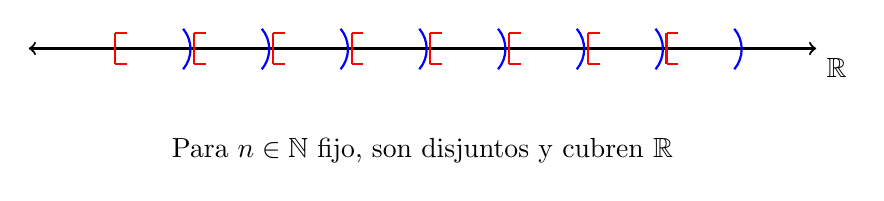
\begin{tikzpicture}
        % Draw the number line
        \draw[thick,<->] (-5,0) -- (5,0) node[anchor=north west] {$\R$};

        % Draw the dyadic intervals of order n=3
        \foreach \j in {-4,...,3} {
            % Draw interval [
            \draw[-, red, thick] (\j+0.1, -0.2) -- (\j+0.1, 0.2);
            \draw[-, red, thick] (\j+0.1, -0.2) -- (\j+0.25, -0.2);
            \draw[-, red, thick] (\j+0.1, 0.2) -- (\j+0.25, 0.2);

            %Draw interval )
            \draw[-, blue, thick] (\j+0.96, 0.25) arc [start angle =40, end angle = -40, radius=0.4];
        }

        % Label the intervals
        \node at (0,-1.3) {Para $n \in \N$ fijo, son disjuntos y cubren $\R$};
    \end{tikzpicture}
\end{center}

\vspace{2mm}
Si $I$ es un intervalo diádico de orden $n$ y $J$ es un intervalo diádico
de orden $m \in \N$ con $m \leq n$: entonces se cumple:
\begin{align*}
    \bullet \hspace{2mm} \text{O bien } I \subsetneq J &&
    \bullet \hspace{2mm} \text{O bien } I \cap J = \varnothing
\end{align*}
La siguiente figura ilustra este hecho:
\vspace{2mm}
\begin{center}
    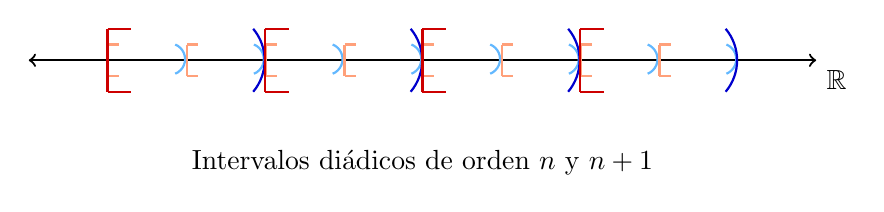
\begin{tikzpicture}
        % Draw the number line
        \draw[thick,<->] (-5,0) -- (5,0) node[anchor=north west] {$\R$};

        % Draw the dyadic intervals of order n=3
        \foreach \j in {-4,...,3} {
            % Draw interval [
            \draw[-, LightSalmon1, thick] (\j+0.01, -0.2) -- (\j+0.01, 0.2);
            \draw[-, LightSalmon1, thick] (\j+0.01, -0.2) -- (\j+0.15, -0.2);
            \draw[-, LightSalmon1, thick] (\j+0.01, 0.2) -- (\j+0.15, 0.2);

            %Draw interval )
            \draw[-, SteelBlue1, thick] (\j+0.86, 0.2) arc [start angle =68, end angle = -68, radius=0.2];
        }

        \foreach \j in {-4, -2, 0, 2} {
            % Draw interval [
            \draw[-, Red3, thick] (\j, -0.4) -- (\j, 0.4);
            \draw[-, Red3, thick] (\j, -0.4) -- (\j+0.3, -0.4);
            \draw[-, Red3, thick] (\j, 0.4) -- (\j+0.3, 0.4);

            %Draw interval )
            \draw[-, Blue3, thick] (\j+1.85, 0.4) arc [start angle =40, end angle = -40, radius=0.6222];
        }
        

        % Label the intervals
        \node at (0,-1.3) {Intervalos diádicos de orden $n$ y $n+1$};
    \end{tikzpicture}
\end{center}

\vspace{6mm}
\result{Definición de cubo diádico}
\hspace{3mm}
Llamamos "cubo diádico de $\R^N$ de orden $n$" con $n, N \in \N$ a cualquier conjunto de
la forma $I_1, \times I_2 \times \ldots \times I_N$ donde cada $I_i$ es un intervalo diádico de orden $n$.

\vspace{2mm} \noindent
Denotaremos por $\mathcal{F}_n$ al conjunto de todos los cubos diádicos de orden $n$ en $\R^N$.

\vspace{4mm}
\result{Propiedades de los cubos diádicos}
\hspace{3mm} Los cubos diádicos de orned $n$ son numerables (consecuencia de la definición y de los resultados anteriores).
Además, son disjuntos o coinciden; es decir:
\begin{align*}
    \left.
    \begin{array}{l}
        C \in \mathcal{F}_n \\
        D \in \mathcal{F}_n \\
        C \neq D
    \end{array}
    \right\}
    \Rightarrow C \cap D = \varnothing
\end{align*}
Como $C,D \in \mathcal{F}_m$, han de ser de la siguiente forma:
\vspace{-2mm}
\begin{align*}
    C = I_1 \times \ldots \times I_n &&
    D = J_1 \times \ldots \times J_n
\end{align*} \\[-5ex]
donde los $I_i$ y los $J_j$ son intervalos diádicos de orden $n$.
Por hipótesis, $C \neq D$ luego ha de existir cierto $k \in \{1, \ldots, n\}$
tal que $I_k \neq J_k$. Por las \hyperref[subsubsection:0.13]{propiedades de los intervalos diádicos},
sabemos que esto implica que $I_k \cap J_k = \varnothing$. Esto a su vez implica que $C \cap D = \varnothing $.
\end{document}